\chapter{評価}
\label{evaluation}

本章では、~\ref{implementation}章で述べたTreeSwiftを用いて、現行のSwiftコンパイラとその構文解析器の実行部分LOCの比較評価を行う。

\section{評価手法}
\label{evaluation:method}

本節では、現行のSwiftコンパイラとTreeSwiftについてその構文解析器の実行部分LOCを評価するための具体的な方法について述べる。

まず、現行のSwiftコンパイラでは、もともと用意されている構文解析のみを実行するオプションをつけるだけでなく、通常そのオプションと共に有効化されるASTの表示機能をコメントアウトすることで、構文解析のみが確実に実行されるように調整する。
また、コンパイラを読み込むデバッガは両コンパイラ共にLLDBのバージョン340.4.119を使用している。
具体的に評価で使用しているSwiftコンパイラおよびその実行時オプションの詳細は表~\ref{table:swift-exe-option}にまとめている。
なお、~\ref{implementation:abstract}節で述べたようにTreeSwiftと現行のSwiftコンパイラではモジュールファイルの形式が異なっており、その点が結果に影響する可能性があるため、計測時にはコンパイラへ標準ライブラリのパスを与えず、モジュールファイルの解析に関する部分が計測対象に含まれないようにしている。

\begin{table}[!hbtp]
    \begin{center}
        \caption{評価に使用したSwiftコンパイラの詳細情報}
        \begin{tabular}{|p{0.3\linewidth}|p{0.65\linewidth}|}
            \hline
            バージョン & swift-2.2-SNAPSHOT-2015-12-31-a からASTの表示をコメントアウトしたもの\\
            \hline
            実行時に使用するオプション & -frontend -dump-parse\\
            \hline
        \end{tabular}
        \label{table:swift-exe-option}
    \end{center}
\end{table}

計測時にコンパイラに読ませるSwiftプログラムにはApple社が提供するプログラミング言語Swiftのチュートリアル~\cite{swift-tour}で用いられている7つのサンプルプログラムを使用する。
ただし、これらのサンプルプログラム中に含まれていた文字リテラル中への式の埋め込みとクロージャを引数に取る関数呼び出しにおける括弧の省略という2つの構文についてはTreeSwiftが対応していないため、同じ意味を持つ明示的な文字列への変換および文字の結合と括弧付きの呼び出しという異なる構文に変更している。

各プログラムの概要を表~\ref{table:measure-sample-programs}にまとめた。
これらのプログラムはチュートリアルという特性上それぞれ異なるSwiftの基本的な機能を使用している上、プログラムで使用される変数や型に使用する名前や値、処理の構造には実際のソフトウェアを想定した現実的なものが選ばれているため、様々な構文について別々にかつ実際のソフトウェアでよく用いられるであろう箇所にフォーカスした計測ができると期待できる。

\begin{table}[!hbtp]
    \begin{center}
        \caption{計測に使用するSwiftプログラム}
        \begin{tabular}{|p{0.4\linewidth}|p{0.1\linewidth}|p{0.45\linewidth}|}
            \hline
            ファイル名 & コメントや空行を除いた行数 & プログラムの概要\\
            \hline
            \hline
            simple\_values.swift & 25 & 変数の定義と使用、文字・数値・配列・辞書リテラルの使用について説明されている。\\
            \hline
            control\_flow.swift & 67 & 分岐や繰り返しについて、Swiftに特徴的なオプショナル値やパターンマッチと組み合わせた例を中心に説明されている。\\
            \hline
            functions\_and\_closures.swift & 69 & 関数の定義と使用について、基本的なものから可変長引数やクロージャを用いた高階関数の呼び出しなどの応用的なものまでが説明されている。\\
            \hline
            objects\_and\_classes.swift & 82 & クラスとそのインスタンス化、継承、関数のオーバーライドなどのSwiftにおけるオブジェクト指向プログラミングについて説明されている。\\
            \hline
            enumerations\_and\_structures.swift & 62 & 構造体とSwiftに特徴的な関数や関連型などを持つ事のできる列挙体についてその宣言方法と使い方が説明されている。\\
            \hline
            protocols\_and\_extensions.swift & 33 & 存在型や型拡張によるクラスや構造体の分類および拡張について説明されている。\\
            \hline
            generics.swift & 25 & 型パラメータ多相を用いた関数や列挙体の宣言方法とその使用方法について説明されている。\\
            \hline
        \end{tabular}
        \label{table:measure-sample-programs}
    \end{center}
\end{table}

\section{計測}
\label{evaluation:measure}

まず、表~\ref{table:complexity-measure}の各プログラムをコンパイルした場合それぞれについて~\ref{evaluation:method}節で説明した方法を用いて実行部分LOCを計測した。
表~\ref{table:loc-result}がその結果および現行のSwiftコンパイラの結果(表中Swift)とTreeSwiftの結果(表中TreeSwift)の比の一覧である。
単純に計測結果だけを見ると、プログラムのコンパイルに要した行数は現行のSwiftコンパイラの方が2$\sim$3倍近く多い。
ただし、TreeSwiftではSwiftコンパイラとして必要な構文解析以外の処理が全て実装されているわけではないため、SwiftコンパイラにおいてはASTの検査など後の処理のための準備が行われており、実行部分LOCがSelf-host化による差だけでなく、その差によって大きく算出されている可能性がある。

そのため、次に各コンパイラの実行部分LOCをその行が書かれているソースコードのファイルごとに分けた上で、構文解析の本体を構成するファイル群(構文解析ファイル群)、ASTを構成するファイル群(ASTファイル群)およびその他のファイル群ごとに集計しなおした。
なお、その他のファイル群にはコンパイラ内の各所から共通で使用されるユーティリティやASTから間接的に使用される構文解析後の処理ステップ用のデータ構造などが含まれている。

表~\ref{table:loc-swift-per-file}および表~\ref{table:loc-treeswift-per-file}はコンパイラごとにそのファイル群ごとの再集計を行った結果であり、図~\ref{img:parse-loc-result}および図~\ref{img:ast-loc-result}はそれらの値の内、構文解析ファイル群とASTファイル群それぞれの実行部分LOCについて現行のSwiftコンパイラのものとTreeSwiftのものを同じグラフ上にプロットしたものである。
また、構文解析ファイル群については後の考察のために各コンパイラにおける実行部分LOCの差と現行のSwiftコンパイラの実行部分LOCに対する差の割合を表~\ref{table:parse-loc-arith}にまとめた。

\begin{table}[!hbtp]
    \begin{center}
        \caption{各コンパイラにおける実行部分LOCの計測結果}
        \begin{tabular}{|p{0.4\linewidth}|p{0.15\linewidth}|p{0.15\linewidth}|p{0.15\linewidth}|}
            \hline
            対象プログラム & Swift & TreeSwift & 比\\
            \hline
            \hline
            simple\_values.swift & 4188 & 1928 & 2.172\\
            \hline
            control\_flow.swift & 5347 & 2226 & 2.402\\
            \hline
            functions\_and\_closures.swift & 5819 & 2187 & 2.661\\
            \hline
            objects\_and\_classes.swift & 5937 & 2122 & 2.798\\
            \hline
            enumerations\_and\_structures.swift & 5762 & 2258 & 2.552\\
            \hline
            protocols\_and\_extensions.swift & 5598 & 2132 & 2.626\\
            \hline
            generics.swift & 5887 & 2233 & 2.636\\
            \hline
        \end{tabular}
        \label{table:loc-result}
    \end{center}
\end{table}

\begin{table}[!hbtp]
    \begin{center}
        \caption{現行のSwiftコンパイラについてファイル群ごとに実行部分LOCを再集計した結果}
        \begin{tabular}{|p{0.4\linewidth}|p{0.15\linewidth}|p{0.15\linewidth}|p{0.15\linewidth}|}
            \hline
            対象プログラム & 構文解析ファイル群 & ASTファイル群 & その他のファイル群\\
            \hline
            \hline
            simple\_values.swift & 1148 & 1263 & 1777\\
            \hline
            control\_flow.swift & 1569 & 1816 & 1962\\
            \hline
            functions\_and\_closures.swift & 1783 & 1982 & 2054\\
            \hline
            objects\_and\_classes.swift & 1934 & 1970 & 2033\\
            \hline
            enumerations\_and\_structures.swift & 1858 & 1886 & 2018\\
            \hline
            protocols\_and\_extensions.swift & 1781 & 1851 & 1966\\
            \hline
            generics.swift & 1897 & 1934 & 2056\\
            \hline
        \end{tabular}
        \label{table:loc-swift-per-file}
    \end{center}
\end{table}

\begin{table}[!hbtp]
    \begin{center}
        \caption{TreeSwiftについてファイル群ごとに実行部分LOCを再集計した結果}
        \begin{tabular}{|p{0.4\linewidth}|p{0.15\linewidth}|p{0.15\linewidth}|p{0.15\linewidth}|}
            \hline
            対象プログラム & 構文解析ファイル群 & ASTファイル群 & その他のファイル群\\
            \hline
            \hline
            simple\_values.swift & 376 & 1457 & 95\\
            \hline
            control\_flow.swift & 433 & 1698 & 95\\
            \hline
            functions\_and\_closures.swift & 448 & 1644 & 95\\
            \hline
            objects\_and\_classes.swift & 437 & 1590 & 95\\
            \hline
            enumerations\_and\_structures.swift & 505 & 1658 & 95\\
            \hline
            protocols\_and\_extensions.swift & 493 & 1544 & 95\\
            \hline
            generics.swift & 481 & 1657 & 95\\
            \hline
        \end{tabular}
        \label{table:loc-treeswift-per-file}
    \end{center}
\end{table}

\begin{figure}
    \begin{center}
        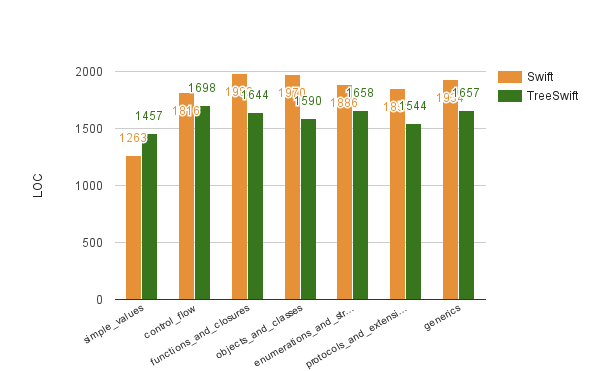
\includegraphics[scale=0.8]{./img/parse_loc_result.png}
        \caption{両コンパイラの構文解析ファイル群の実行部分LOCの比較}
        \label{img:parse-loc-result}
    \end{center}
\end{figure}

\begin{figure}
    \begin{center}
        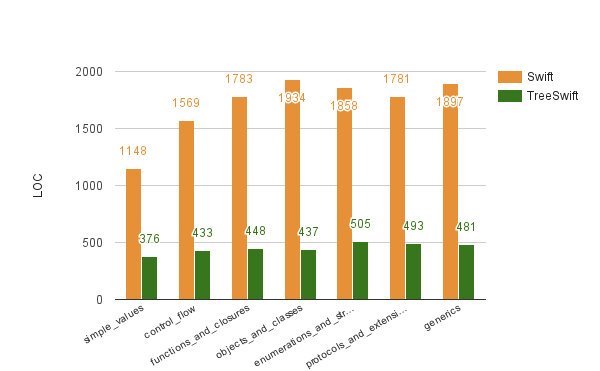
\includegraphics[scale=0.8]{./img/ast_loc_result.png}
        \caption{両コンパイラのASTファイル群の実行部分LOCの比較}
        \label{img:ast-loc-result}
    \end{center}
\end{figure}

\begin{table}[!hbtp]
    \begin{center}
        \caption{各コンパイラの構文解析本体ファイルに対象を絞った実行部分LOCの差と比}
        \begin{tabular}{|p{0.45\linewidth}|p{0.225\linewidth}|p{0.225\linewidth}|}
            \hline
            対象プログラム & 差 & SwiftからのLOC減少率\\
            \hline
            \hline
            simple\_values.swift & -194 & -16.9 \%\\
            \hline
            control\_flow.swift & 118 & 7.52 \%\\
            \hline
            functions\_and\_closures.swift & 338 & 19.0 \%\\
            \hline
            objects\_and\_classes.swift & 380 & 19.6 \%\\
            \hline
            enumerations\_and\_structures.swift & 228 & 12.3 \%\\
            \hline
            protocols\_and\_extensions.swift & 307 & 17.2 \%\\
            \hline
            generics.swift & 277 & 14.6 \%\\
            \hline
        \end{tabular}
        \label{table:parse-loc-arith}
    \end{center}
\end{table}

\subsection{考察}

まず、表~\ref{table:loc-result}の全体における実行部分LOCで両コンパイラに異様に大きな差を与えていた原因は表~\ref{table:loc-swift-per-file}の実行部分LOCをファイル群ごとに再集計した結果から、構文解析ファイル群ではなく、それ以外のファイル群に含まれるプログラムにあると考えられる。
実際、現行のSwiftコンパイラはその後に控えるSIL生成のためにASTを走査して正当性の確認を行ったり、Swiftプログラムの構文からSIL生成用の付帯情報が構文解析時に生成されるようにしており、それらのTreeSwiftに存在しない機能を提供するためのプログラムが実行部分LOCの大きな差を生んでいると見られる。
なお、表~\ref{table:loc-treeswift-per-file}においてその他のファイル群の実行部分LOCが同じ値となっているのは、TreeSwiftではそうした追加情報の生成やASTの正当性確認を行っておらず、その他のファイルがコンパイラ全体で使用されるファイルI/Oの仕組みなどを提供する基本ツールだけで構成されており、構文にかかわらず同じように使用されているからである。

しかし、図~\ref{img:parse-loc-result}にあるそうした部分を差っ引いた構文解析ファイル群の結果のみについて見ても、simple\_values.swift以外のプログラム全てでTreeSwiftの方が低い実行部分LOCを記録している。
特にこの差を作り出していると考えられる原因の1つが、両コンパイラにおける分岐構文の使用傾向の差異である。
表~\ref{table:branching-method-swift}および表~\ref{table:branching-method-treeswift}は構文解析ファイル群の実行部分LOCの算出元となっている行の内、分岐構文の使用されている行がどれだけ存在するかを調べたものである。
なお、分岐構文としては現行のSwiftコンパイラではif文とswitch文とassert文、TreeSwiftではif文とswitch文とguard文をそれぞれ対象としている。

これらの表に見られる通り、現行のSwiftコンパイラにおいてはswitch文に対してif文が多く使用されているのに比べて、TreeSwiftではif文の使用量が減り、代わりにswitch文の使用量が増加している。
これは、Swiftの持つ強力なパターンマッチや列挙型によって、C++では異なる分岐文で別個に処理されていたものを同一のswitch文で使用できるようになったためだと考えられる。
Swiftのパターンマッチは条件判定と同時に列挙型やタプルなどの内部構造を分解して変数に束縛する役割を果たすため、switch文への移行は複数の条件文をまとめた上で変数の宣言や代入に関する行を削減することに繋がり、結果として実行部分LOCに減少につながっていたと考えられる。

また、simple\_values.swiftのみにおいてTreeSwiftの実行部分LOCが大きくなっていたのは、~\ref{implementation:abstract}節で述べたように、TreeSwiftでは構文解析のステップを簡略化するために字句解析器が比較して複雑なアルゴリズムを採用しているためだと思われる。
これは、7つの対象プログラムについてSwiftの構文解析本体ファイルのみを対象とした実行部分LOCの標本分散は約53874であるのに対して、TreeSwiftでは約5930と低く、TreeSwiftの方が全てのプログラムで共通して実行されている部分が多くの部分を占めていることからも考察できる。

以上の考察より、表~\ref{table:parse-loc-arith}中の結果はSwiftコンパイラをSelf-host化したことによる効果を充分表しており、Self-host化によってSwiftコンパイラの実行部分LOCを評価に用いたプログラムで平均して10.47\%減少させることができたことがわかる。

\begin{table}[!hbtp]
    \begin{center}
        \caption{Swiftにおける構文解析ファイル群の実行部分中の分岐構文の行数}
        \begin{tabular}{|p{0.4\linewidth}|p{0.15\linewidth}|p{0.15\linewidth}|p{0.15\linewidth}|}
            \hline
            対象プログラム & if文 & switch文 & assert文\\
            \hline
            \hline
            simple\_values.swift & 266 & 22 & 33\\
            \hline
            control\_flow.swift & 392 & 28 & 43\\
            \hline
            functions\_and\_closures.swift & 432 & 28 & 46\\
            \hline
            objects\_and\_classes.swift & 449 & 28 & 37\\
            \hline
            enumerations\_and\_structures.swift & 407 & 26 & 38\\
            \hline
            protocols\_and\_extensions.swift & 407 & 27 & 35\\
            \hline
            generics.swift & 436 & 26 & 43\\
            \hline
        \end{tabular}
        \label{table:branching-method-swift}
    \end{center}
\end{table}

\begin{table}[!hbtp]
    \begin{center}
        \caption{TreeSwiftにおける構文解析ファイル群の実行部分中の分岐構文の行数}
        \begin{tabular}{|p{0.4\linewidth}|p{0.15\linewidth}|p{0.15\linewidth}|p{0.15\linewidth}|}
            \hline
            対象プログラム & if文 & switch文 & guard文\\
            \hline
            \hline
            simple\_values.swift & 193 & 60 & 19\\
            \hline
            control\_flow.swift & 223 & 68 & 22\\
            \hline
            functions\_and\_closures.swift & 206 & 69 & 21\\
            \hline
            objects\_and\_classes.swift & 208 & 69 & 23\\
            \hline
            enumerations\_and\_structures.swift & 219 & 71 & 26\\
            \hline
            protocols\_and\_extensions.swift & 201 & 64 & 25\\
            \hline
            generics.swift & 214 & 70 & 26\\
            \hline
        \end{tabular}
        \label{table:branching-method-treeswift}
    \end{center}
\end{table}

%%% Local Variables:
%%% mode: japanese-latex
%%% TeX-master: "../thesis"
%%% End:
